% !TEX root = ../main.tex

\chapter{Machine learning state of the art} \label{chap:state-of-the-art}

\begin{displayquote}
\textit{This chapter defines the concept of machine learning and presents a comprehensive overview of the algorithms and models that are more relevant with the biomedical data science applications described in Part II.}
%\section{} \label{sec:machine_learning}
\end{displayquote}

The term \textit{Machine Learning} (ML) first appeared in the late 50's in the field of computer science and it is now becoming a buzzword used in several contexts spanning from particle physics and astronomy to medicine and social sciences~\cite{service2017ai}.
With a simple search on Google Trends\footnote{\url{https://trends.google.com}} it is possible to roughly quantify the pervasiveness of this term on the Internet in the last few years. From Figure~\ref{fig:google_trend_ML} we can see that the interest toward both the terms \textit{machine learning} and \textit{data science} is growing, with the first consistently superior to the second.

\begin{figure}[h!]
  \centering
    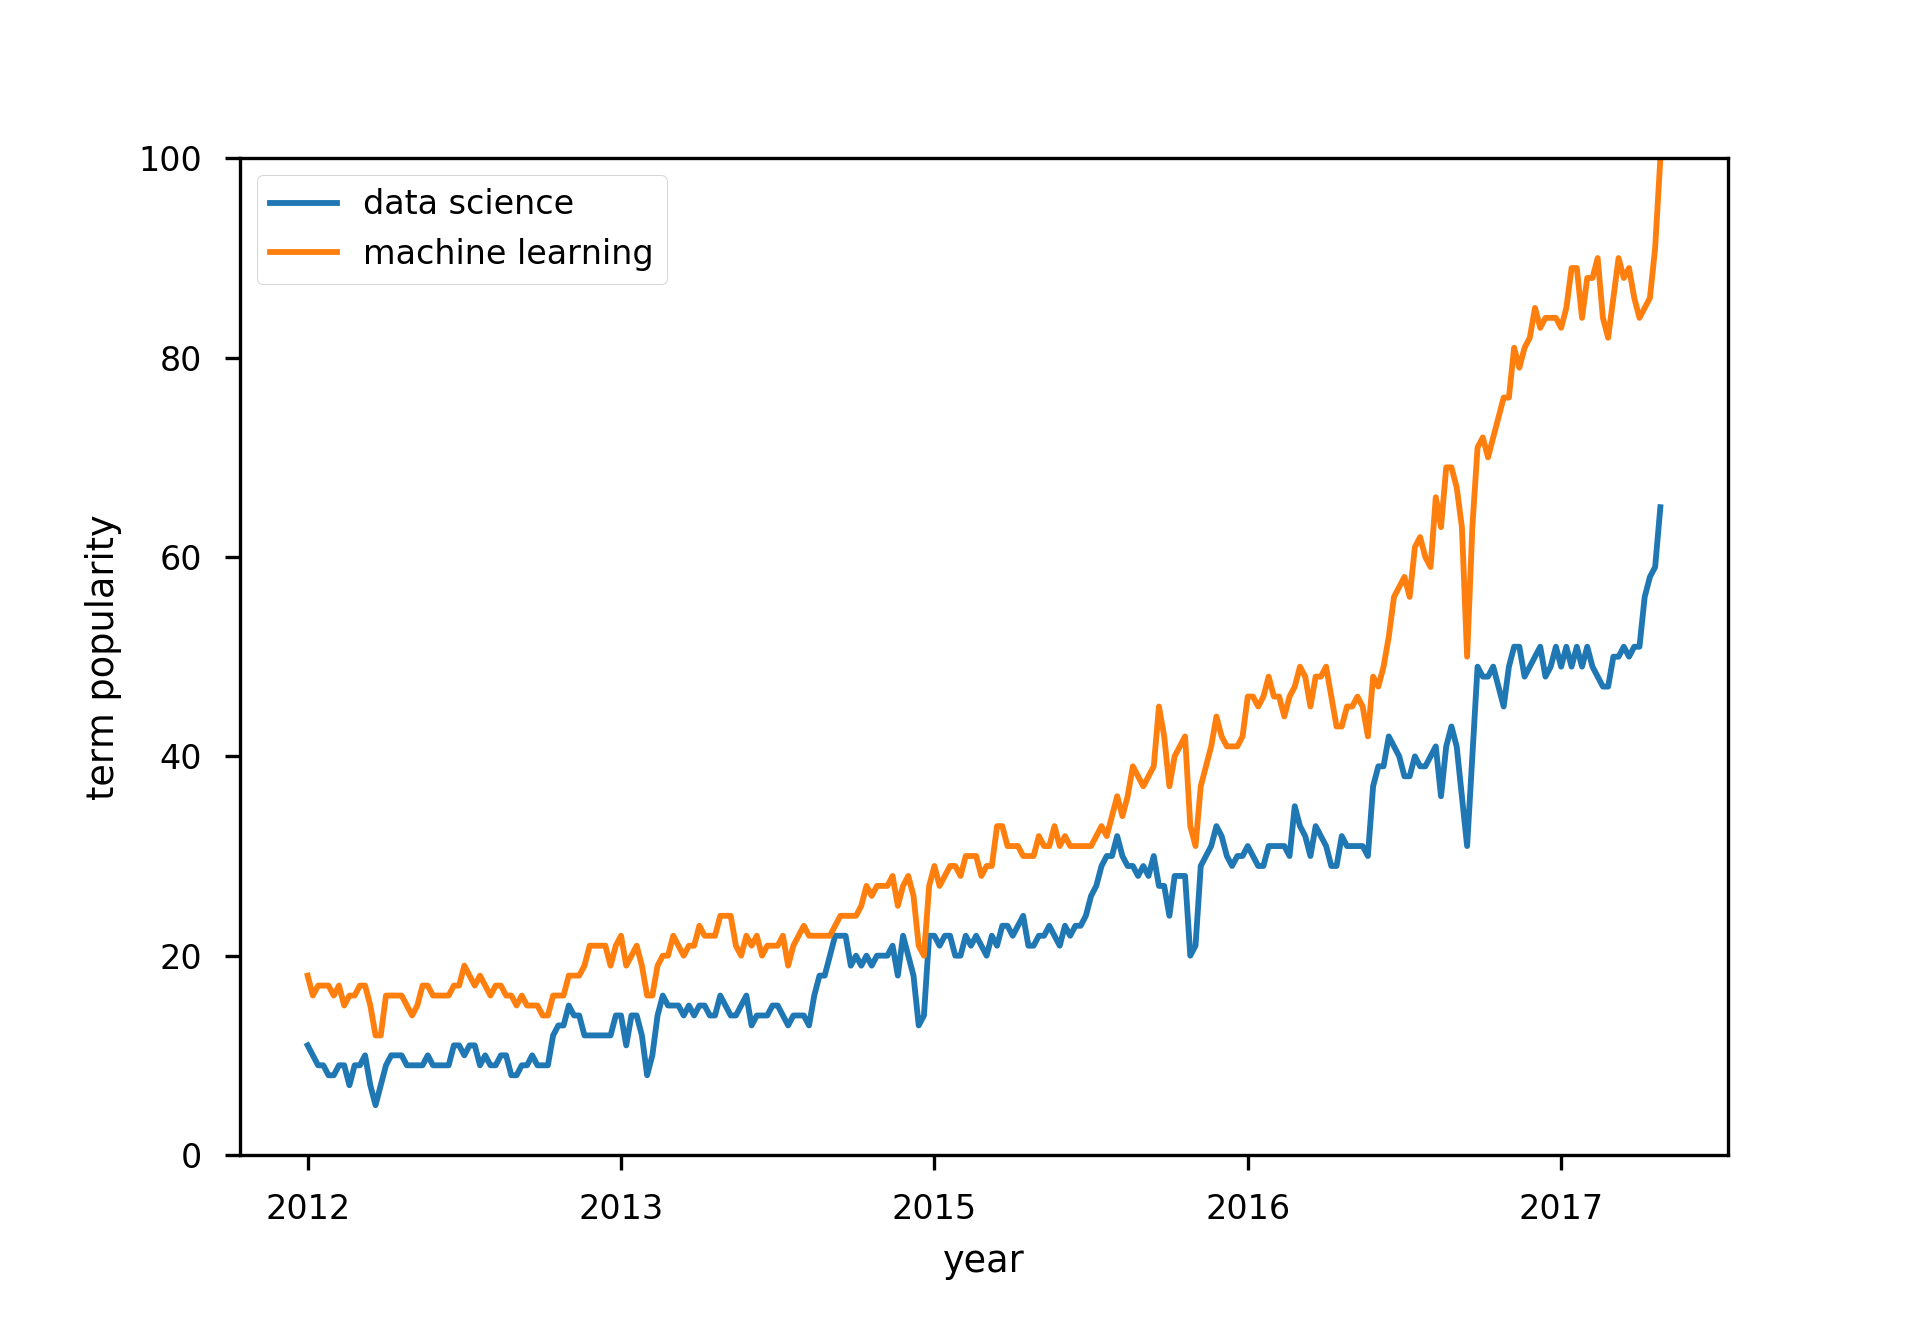
\includegraphics[width=0.8\textwidth]{part1/google_trends_MLDS.png}
  \caption{The Internet popularity over the past five years of two terms: \textit{data science} and \textit{machine learning}. The vertical axis represents the number of Google searches of an input term normalized with respect to its maximum (source: Google Trends).} \label{fig:google_trend_ML}
\end{figure}

A partial explanation to this phenomenon can be found in a recent article published on Science~\cite{appenzeller2017revolution}, where the authors observed how the explosion in modern data collection abilities is leading to a new \textit{scientific revolution}.
Biomedical applications are prototypical in this sense. For instance, raw data acquired by a genome sequencer from a single individual weight around 140 GB~\cite{marx2013biology} and a 3D reconstruction of cardiac MRI acquisition need around 20 GB. Currently, an average hospital requires more than 665 TB of storage.
%the typical resolution of MRI images is currently $512 \times 512$
Such massive amounts of data have long overwhelmed human analysis and insights potential. This makes ML a key element for clinicians and scientists trying to make sense of large-scale observations.

But, what is \textit{machine learning}? And how does it differ from statistics?

A unique answer to this question may not be easy to provide. In fact, ML can be defined in different ways and from several standpoints. Let's see three remarkable examples.

\begin{enumerate}
  \item Kevin P. Murphy in its \emph{Machine Learning - A Probabilistic Perspective}~\cite{murphy2012machine} defines machine learning as follows.

  \begin{displayquote}
  "[...] \emph{a set of methods that can automatically detect patterns in data, and then use the uncovered patterns to predict future data, or to perform other kinds of decision making under uncertainty} [...]"
  \end{displayquote}

  \item Trevor Hastie, a well-known applied statistician, in a famous seminar\footnote{part of Data Science @ Stanford Seminar series (source: \url{https://goo.gl/UFgqxU}).}, held in October 2015 at the Stanford University, gave the following three definitions.

  \begin{displayquote}
    \begin{itemize}
      \item[] \emph{{\bf Machine Learning} constructs algorithms that can learn from data.}
      \item[] \emph{{\bf Statistical Learning}  is a branch of applied statistics that emerged in response to machine learning, emphasizing statistical models and assessment of uncertainty.}
      \item[] \emph{{\bf Data Science}  is the extraction of knowledge from data, using ideas from mathematics, statistics, machine learning, computer science, engineering...}
    \end{itemize}
  \end{displayquote}

  \item Carl E. Rasmussen in the preface of its renowned \emph{Gaussian Processes for Machine Learning}~\cite{rasmussen2006gaussian} introduces the difference between statistics and ML as follows.

  \begin{displayquote}
    "\emph{in statistics a prime focus is often in understanding the data and relationships in terms of models giving approximate summaries such as linear relations or independencies. In contrast, the goals in machine learning are primarily to make predictions as accurately as possible and to understand the behaviour of learning algorithms}"
  \end{displayquote}

\end{enumerate}

It looks like each author, according to his background, expertise and experience, provides a slightly different definition of ML. Trying to summarize these three standpoints, we can say that \emph{ML is an interdisciplinary field that borrows the concept of data-driven model from statistics in order to devise algorithms that can exploit hidden patterns in current data and make accurate predictions on future data}.

As of today ML is the workhorse of data science.


  \section{Supervised learning} \label{subsec:supervised_learning}

  Humans are remarkably good at \emph{learning by examples}. When a kid is taught what a pencil looks like, he will be capable of understanding the concept of pencil from a limited number of guided observations. Similarly, when future radiologists are trained to distinguish between healthy tissues from tumors in MRI scans, they will be provided with several annotated biomedical images from which they will be able to generalize.
  The applied learning paradigm is characterized by the presence of two key objects: \textit{data} and \textit{labels}. In the last example, the MRI scans are the data, and their annotations (\eg tumor vs healthy tissue) are the labels.

  Supervised learning is the branch of ML in which predictive models are trained on labeled data. In the ML jargon, and in this thesis, one usually refers to \textit{data} as collections of \textit{samples} described by an arbitrarily large number of \textit{predictors} (\textit{features}) that are used as \textit{input} in a training process having labels as \textit{output}.

  Input samples throughout this thesis are represented as $d$-dimensional vectors $\bm{x}$ belonging to an input space $\mathcal{X}$, where $\mathcal{X}\subseteq\mathbb{R}^d$ and labels are represented with the variable $y$ belonging to an output space $\mathcal{Y}$.
  The nature of $\mathcal{Y}$ defines the learning task as \textit{binary classification} if  $\mathcal{Y} = \{-1,+1\}$, \textit{multiclass classification} if $\mathcal{Y} = \{1,2,\dots,k\}$,
  \textit{regression} if $\mathcal{Y}\subseteq\mathds{R}$ and
  \textit{vector-valued regression} if $\mathcal{Y}\subseteq\mathds{R}^k$.
%  In the second part of this thesis each of these learning problems will be faced.
  The remainder of this section summarizes the methods that are most relevant with the data-driven strategies adopted to tackle the biomedical data science challenges described in the second part of in this thesis.

%    \subsubsection{The optimization problem} \label{subsubsec:supevised_optimization}

    Given a set of input-output pairs $\{\bm{x}_i, y_i\}_{i=1}^n$, supervised learning methods aim at finding a function of the inputs $f(\bm{x})$ that approximates the output $y$. This translates into the minimization problem defined in Equation~\eqref{eq:loss}.
    \todo{ERM vs MLE/MAP}

    \begin{equation}\label{eq:loss}
      \min_f \frac{1}{n}\sum_{i=1}^n V(f(\bm{x}_i),y_i) %+ \lambda R(f)
    \end{equation}

    The loss function $V(f(\bm{x}),y)$ can be seen as a measure of \textit{adherence} to the available training data. Several loss functions for regression and classification problems were proposed; Table~\ref{tab:losses} defines the most commonly adopted in biomedical studies while their visual representation is presented in Figure~\ref{fig:loss}. \todo{Different choices for the loss function imply different ML model, see the remainder of this section + this is possibly ill-posed}
        
     % rubare da BIB
    % In its most classical definition, the aim of modeling is to infer some unknown structure underlying the data.
    The process of identifying a model from a real-world data collection can be very hard. Many unwanted and concurrent factors may be misleading and the result may have poor predictive power. For instance, the acquisition devices may introduce random fluctuations in the measures or the amount of collected samples $n$ may be small with respect to the number of observed variables $d$ which, in turn, may not even be representative of the target phenomenon. From a modeling standpoint, every combination of the factors above can be seen as \textit{noise} affecting the data. Precautions in the model formulation process must be taken in order to achieve solutions that are \textit{robust} to the noise effect. \todo{+overfit +figu}
    \todo{In ML, a model that fits well the training data but performs poorly on new samples is said to be \textit{overfitting} the training set.}
    
    A common strategy to build predictive models out of noisy data is called \textit{regularization}. As the biomedical world is the the main area of interest of this thesis (see Section~\ref{sec:challenges_biomedical}), for each learning algorithm described, particular emphasis will be put on the relevant regularization strategies.    
    In its broader definition regularization is the process of introducing additional information $R(f)$ in order to solve a possibly ill-posed problem \cite{tikhonov1963solution, evgeniou2000regularization}. \todo{Equation~\eqref{eq:lossq:losspen}}
    
     \begin{equation}\label{eq:losspen}
    	\min_f \frac{1}{n}\sum_{i=1}^n V(f(\bm{x}_i),y_i) + \lambda R(f)
    \end{equation}
    
    
    The expected result is a function that fits the training data while having good generalization properties, \ie accurate predictions on previously  \textit{unseen} test data \cite{hastie2009elements}. 
        
    
%    
%    The regularization penalty $R(f)$ imposes stability on the expected function exploiting the available prior knowledge on the problem~\cite{tikhonov1963solution}. More details on $R(f)$ will be given in the next section.

    
    \begin{figure}[!ht]
        \centering
        \subfloat[]{%
            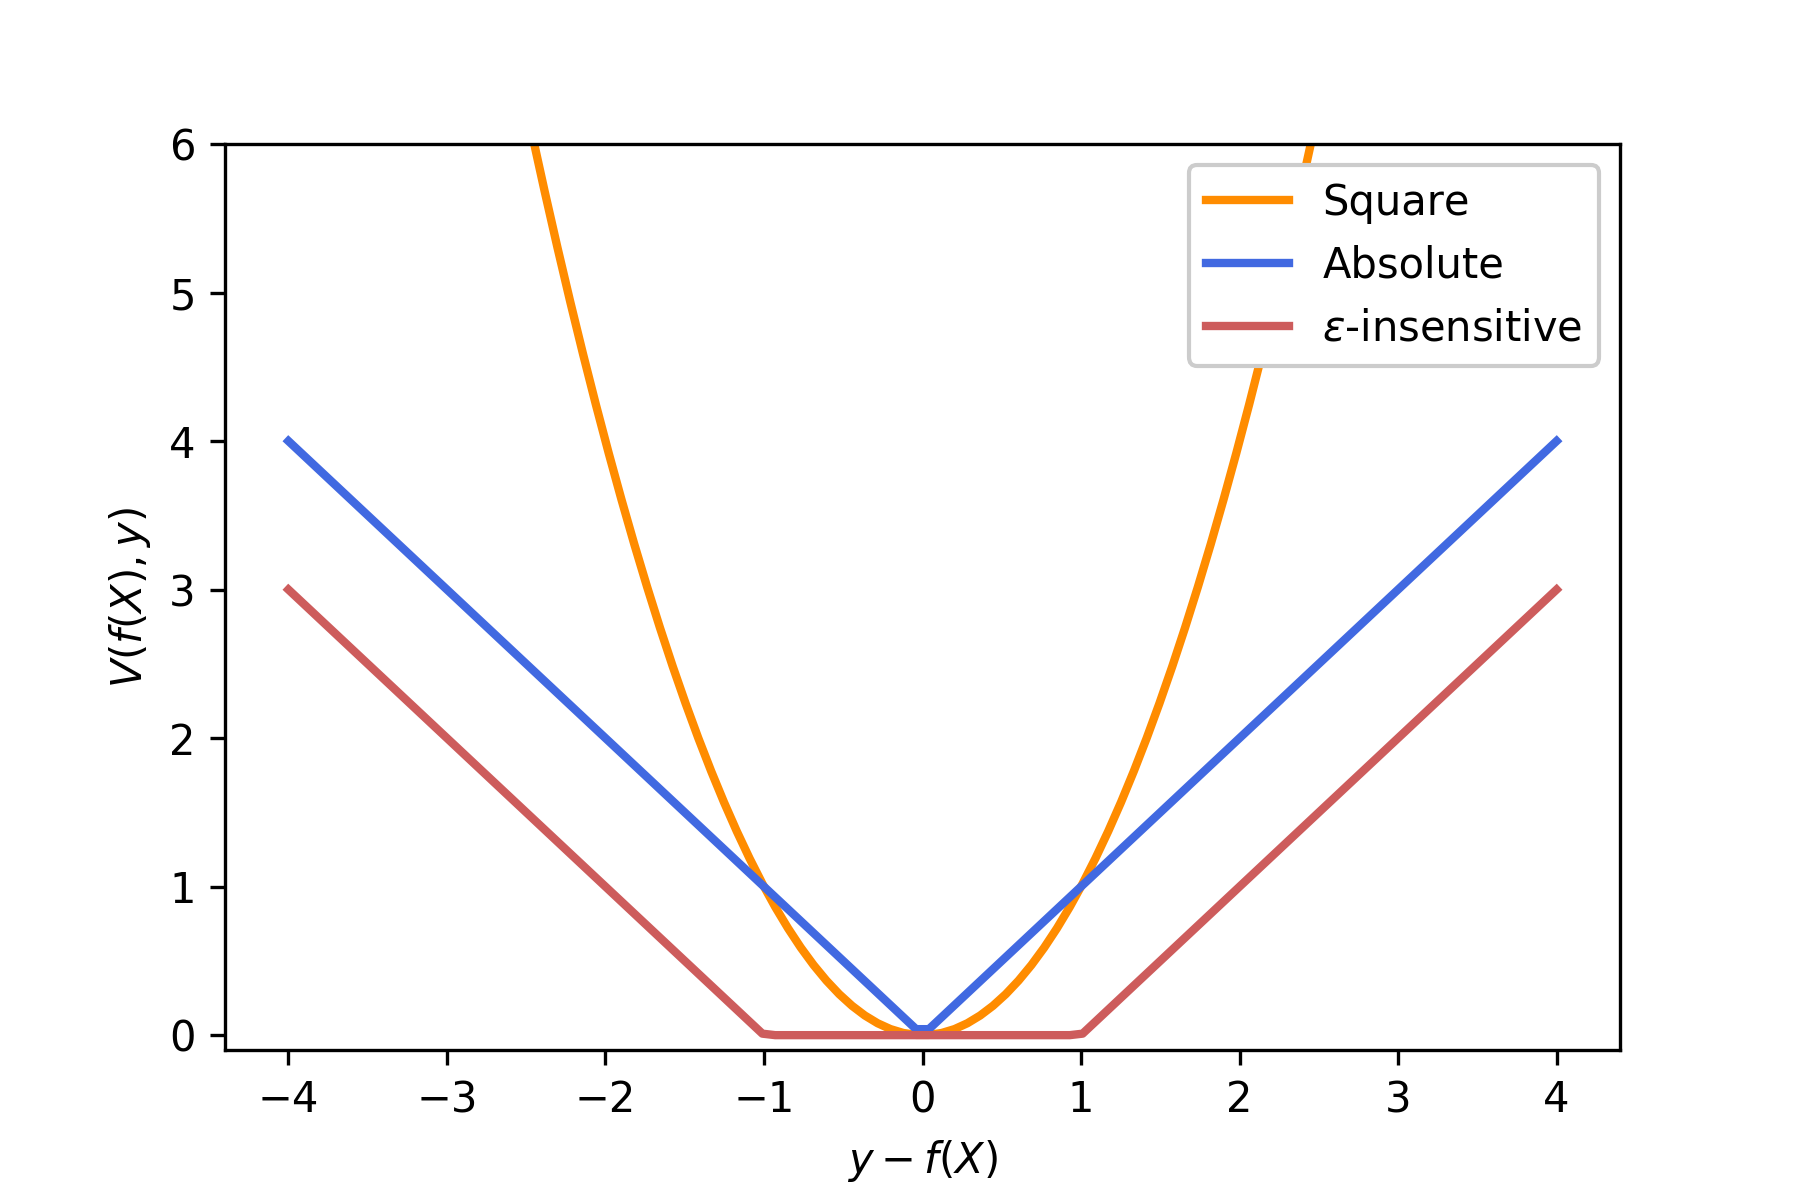
\includegraphics[width=0.5\textwidth]{part1/regression_losses.png}
            \label{fig:regression}%
        }%
        % \hfill%
        \subfloat[]{%
        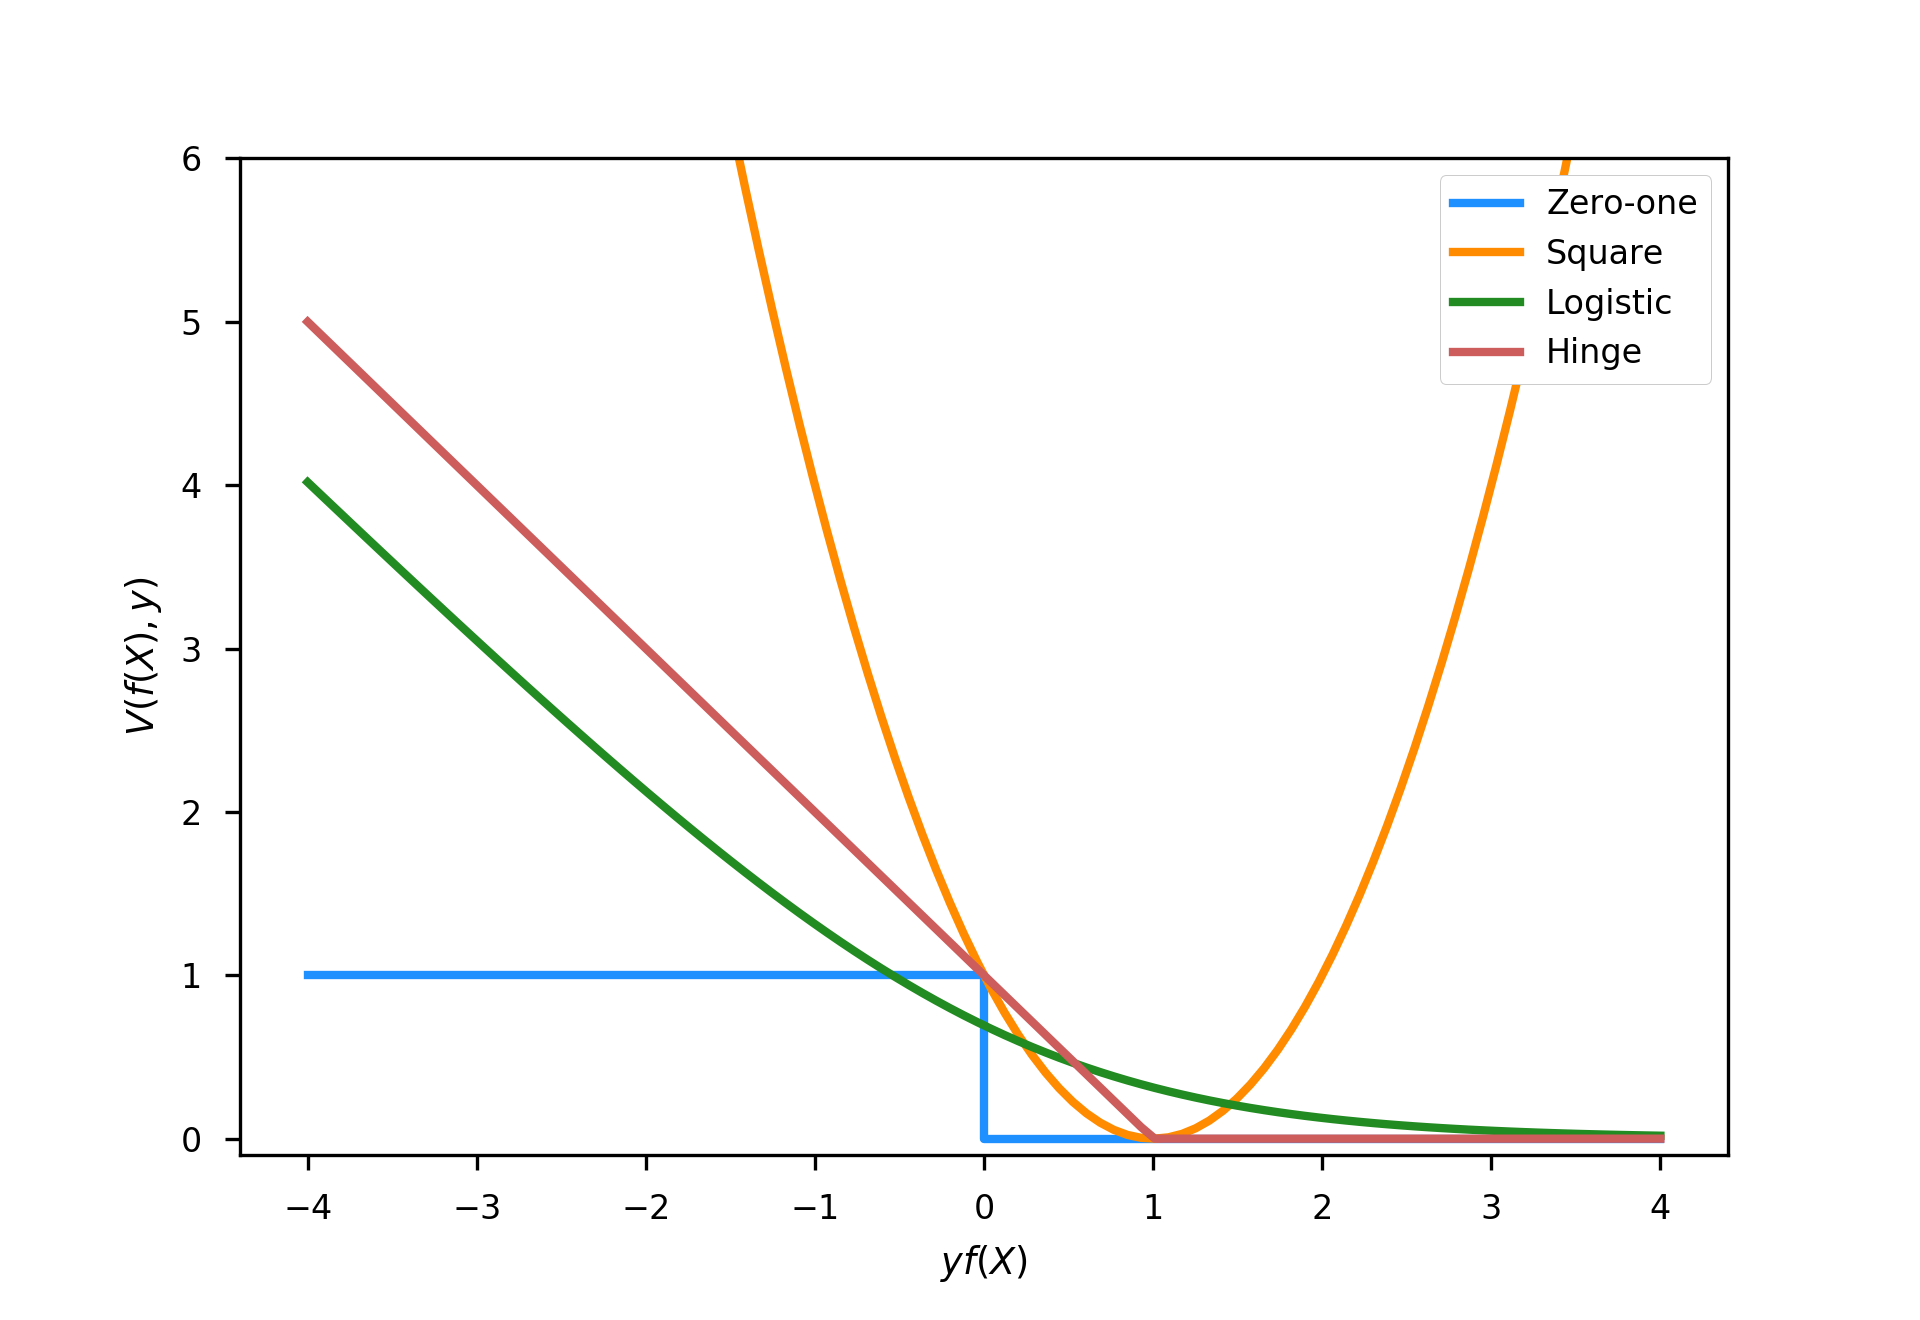
\includegraphics[width=0.5\textwidth]{part1/classification_losses.png} \label{fig:classification}
        }%
        \caption{An overview on the most common loss functions for regression (a) and classification (b) problems plotted against the corresponding prediction error.}\label{fig:loss}
    \end{figure}


    \begin{table}[!ht]
      \centering
      \caption{Definition of the loss functions for regression (top) and classification (bottom) problems represented in Figure~\ref{fig:loss}.}\label{tab:losses}
      \begin{tabular}{@{}ll@{}ll@{}}
        \toprule
        Loss function & $V(f(\bm{x}),y)$  & Learning problem           \\ \midrule
        Square                   & $(y - f(\bm{x}))^2$ & regression \\
        Absolute                 & $|y - f(\bm{x})|$ & regression   \\
        $\epsilon$-insensitive   & $\begin{cases}
            0 & \text{if } |y-f(\bm{x})| < \epsilon\\
            |y-f(\bm{x})| - \epsilon & \text{otherwise}
        \end{cases} $        & regression                 \\
        \midrule
        Zero-one               & $\begin{cases}
            0 & \text{if } y = f(\bm{x})\\
            1 & \text{otherwise}
            \end{cases}$ & classification \\
        Square                 & $(1 - yf(\bm{x}))^2$ & classification  \\
        Logistic                 & $\log(1 + e^{-yf(\bm{x})})$ & classification  \\
        Hinge                 & $|1 - yf(\bm{x})|_+$ & classification  \\
        \bottomrule
      \end{tabular}
    \end{table}

    Supervised learning machines can rely on very different mathematical backgrounds such as generalized linear models, nonlinear deep neural networks, kernels, trees, ensemble of trees, \etc. Nevertheless, disregarding their nature, they all share the common structure defined in Equation~\eqref{eq:losspen}. Although, the posed optimization problems can have very different properties; they can be convex, non-convex, they can include differentiable as well as non-differentiable terms. A rigorous review of the most common optimization problems in ML is beyond the scope of this thesis and can be found here~\cite{boyd2004convex, bach2012optimization, sra2012optimization, nesterov2013introductory}.

       

    \subsection{Regularization methods}
    Regularization methods are a broad class of ML models that include ...

    \subsection{Ensemble methods}

    The key idea behind ensemble methods is to build a prediction model by aggregating a collection of multiple \textit{base learners} that are trained to solve the same problem~\citep{zhou2012ensemble}.

    % FIXME
    \textit{Bagging} is a common ensemble method that consists in fitting multiple models $f_b(\bm{x})$ for $b=1,\dots,B$ each one on a \textit{bootstrap} data set $\{X,\bm{y}\}_b$ obtained from the training set $\{X,\bm{y}\}$ by random sampling with replacement~\citep{hastie2009elements}. For each sample $\bm{x}_i$, the bagging estimate $\hat{f}(\bm{x}_i)$ is obtained by combining the predictions of the base learners $\hat{f}_b(\bm{x}_i)$. In particular, in case of classification tasks, the bagged model selects the most predicted class casting a vote among the $B$ base learners.

    % FIXME
    \textit{Boosting} is another popular ensemble method that, unlike bagging, performs predictions by sequentially fitting a collection of base learner that cast a weighted vote~\citep{hastie2009elements}. At each boosting step, the weight corresponding to samples that were misclassified at the previous iterations increases. Therefore, each successive classifier is somewhat forced to learn the relationships between input and output that were previously missed. From a theoretical standpoint, it would be possible to boost any learning machine, nevertheless boosting methods are mainly used with decision trees as base learners.


    \subsubsection{Random Forests}
    Decision trees are easily interpretable models that recursively partitions the training data into subsets, based on the test of a single feature value at each split (or node). At each iteration, the feature that yields the best split in terms of a pre-selected metric (Gini impurity, information gain or variance reduction) is chosen to create a new node. Decision trees tend to not perform well in practice, which led to the introduction of random forests in 2001~\cite{breiman2001random}.

    Random forests are ensembles of decision trees, each grown on a bootstrap sample from the training data.
    To increase robustness to noise and diversity among the trees, each node is split using the best split among a subset of features randomly chosen at that node.
    The final prediction is made by aggregating the prediction of $m$ trees, either by a majority vote in the case of classification problems, or by averaging predictions in the case of regression problems.
    Random forests are a {\it bagging} approach, which works on the assumption that the variance of individual decision trees can be reduced by averaging trees built on many uncorrelated subsamples.
    By contrast, {\it boosted decision trees} are made by building an iterative collection of decision trees, trained by giving more importance to training examples that were incorrectly classified by the previous trees. \todo{Add use cases for boosted decision trees. $\dots$}

    Random forests can provide several measures of {\it feature importance}, computed by looking at the increase in prediction error % (mean decrease in accuracy; mean decrease in node impurity)
    when data for a feature is permuted while all other features remain unchanged. Feature selection based on random forests if most often performed using one of these measures. However, several techniques for applying regularization to random forests have been proposed. These techniques broadly fall under two categories: (1) cost-complexity pruning, which consists in limiting tree depth, resulting in less complex models~\cite{ishwaran2008random,kulkarni2012pruning}; and (2) Gini index penalization~\cite{deng2013gene, liu2014learning}. In addition,~\cite{joly2012ell1} proposed using an $\ell_1$-norm  to reduce the space-complexity of random forests.

    Random forests naturally handle both numerical and categorical variables, multiple scales, and non-linearities. They also require little parameter tuning. This makes them popular for the analysis of diverse types of biological data, such as gene expression, GWAS data or mass spectrometry~\cite{qi2012random}. Unfortunately, in practice feature selection schemes that rely on them tend to be very unstable~\cite{kursa2014robustness}.

    \subsubsection{Gradient Boosting}
    \textit{Gradient boosting}~\citep{friedman2001greedy}  is one of the most widely applied boosting methods in biological problems.
    %This technique iteratively combines the predictions obtained by several base learners, such as decision trees, into a single model.
    The key idea behind gradient boosting is that, under some general hypothesis on the cost function, boosting can be seen as an iterative gradient method for numerical optimization.
    %In particular, in GB at each boosting step a new base learner is fitted on the residuals obtained at the previous boosting iteration.
    Gradient boosting has several desirable properties~\citep{mayr2014evolution}, such as its capability to learn nonlinear input/output relationship, its ability to embed a feature importance measure (as random forests~\citep{hastie2009elements}) and its stability in case of high-dimensional data~\citep{buehlmann2006boosting}.

    %The consistency of GB in high-dimensional problems was demonstrated in.

    As for any learning machine, boosting methods may suffer of overfitting. The main regularization parameter to control is the number of boosting iterations $M$, \ie the number of base learners, fitted on the training data. This is typically optimized by cross-validated grid-search, or by information criteria-based heuristics~\citep{tutz2006generalized, tutz2007boosting} (see Section~\ref{subsec:model_selection}).

    Regularization in gradient boosting can also be controlled by shrinking the contribution of each base learner by a constant $0<\nu<1$ that controls the learning rate of the boosting procedure~\citep{hastie2009elements}. In order to achieve comparable predictive power, smaller values of $\nu$ imply larger number of $M$, so there is a tradeoff between them.
    As usually the base learners are decision trees, another important parameter to tune is their maximum depth~\citep{hastie2009elements}.

    In a recent paper~\citep{lusa2015boosting}, the authors show that in high-dimensional balanced binary classification problems, if the base learner is likely to overfit the training data, the use of \textit{Stochastic gradient boosting}~\citep{friedman2002stochastic} is preferable. The latter is a modified version of the original method, where each base learner is fitted on a random extraction without resubmission of a fraction $\eta$ of the training data, where $\eta$ is de-facto a regularization parameter to choose.

    Approaches based on gradient boosting classification are used to detect \textit{de novo} mutations showing an improved specificity and sensitivity with respect to state-of-the-art methods~\citep{liu2014gradient}.
    When combined with stability selection~\citep{meinshausen2010stability}, gradient boosting has demonstrated to be a very resourceful method for variable selection, leading to an effective control of the false discovery rate. This strategy was followed to associate overall survival with single-nucleotide polymorphisms of patients affected by cutaneous melanoma~\citep{he2016component} and to detect differentially expressed amino acid pathways in autism spectrum disorder patients~\citep{hofner2015controlling}.

    \todo{consider adding boosting method for cox models...}



%%



    \subsection{Deep learning}
    % I shall not forget that this is Regularization in bio studies, there are plenty of ML in bio studies out there
    Deep Learning (DL) methods are a broad class of machine learning techniques that, starting from raw data, aim at learning a suitable feature representation (see Section~\ref{sec:unsupervised}) and a prediction function, at the same time~\cite{lecun2015deep}. DL methods can be seen as an extension of classical Neural Networks, where the final prediction is achieved by composing several layers of non-linear transformations.
    %The intuition behind DL method is that, starting from raw data, their multi-layer architecture can achieve representations at a more abstract level, capable of achieving high performance in prediction tasks.
    DL architectures can be devised to tackle binary/multi-category classification~\cite{angermueller2016deep, leung2014deep} as well as single/multiple-output regression~\cite{Chen2016GeneEI, ma2015deep} tasks.
    %\todo{microarray gene xpression multi-task regression }

    Many methods fall in this class~\cite{lecun2015deep}, in order to understand them in general, we sketch here the main ideas behind the most basic one: the Multi-Layer Perceptron (MLP), also known as deep feedforward network.
    Typically, MLPs are structured as fully connected graphs organized in \textit{layers} that can be of three different types: \textit{input},  \textit{hidden} and \textit{output} (see Figure~\ref{fig:mlp}). Each node of the graph is called \textit{unit}. The number of units in the input layer matches the dimensionality of the raw data ($d$), while number and type of output units are related to the learning task. The size of the hidden layer, and their number, can be arbitrarily chosen according to the prediction task and the available computational resources.
    In MLPs the information flows through the graph from the input to the output. Each layer $l$ transforms its input data $\bm{x}^{l-1}$ by composing an affine transformation and an activation function $f(\cdot)$ that acts element-wise on its input vector. In other words, defining as $p_{l-i}$ the number of units in the layer $l-i$, the layer $l$ applies the transformation $\bm{x}^{l} = f(\bm{x}^{(l-1)}W_l+b_l)$, where $W_l \in \mathbb{R}^{p_{l-1} \times p_l}$ and $\bm{b} \in \mathbb{R}^{p_l}$ are the weights of the model that are learned from the data. The function $f(\cdot)$ is known as \textit{activation function} and it can be defined in different ways. In classical neural networks, activation functions are modeled as sigmoids (\eg $f(x)=\tanh(x)$, $f(x)=(1+e^{-x})^{-1}$) whilst in modern DL architectures the most used activation function is the Rectified Linear Unit (\ie $f(x)=\max(0,x)$)~\cite{lecun2015deep} .
    % \begin{equation}\label{eq:relu}
    % 	f(\bm{x})=\begin{cases} 0  &\text{for}~~  x <0 \\ x  &\text{for~}~x \geq 0 \end{cases}
    % \end{equation}

    \def\layersep{2.0cm}

\begin{figure}
	\caption{A pictorial representation of the structure of a Multi-Layer Perceptron example with two hidden layers having four and three hidden units, respectively. According to the nature of the output layer, this network topolgy can be adopted either for regression or binary classification problems starting from raw samples in a two-dimensional space.} \label{fig:mlp}
	\centering
	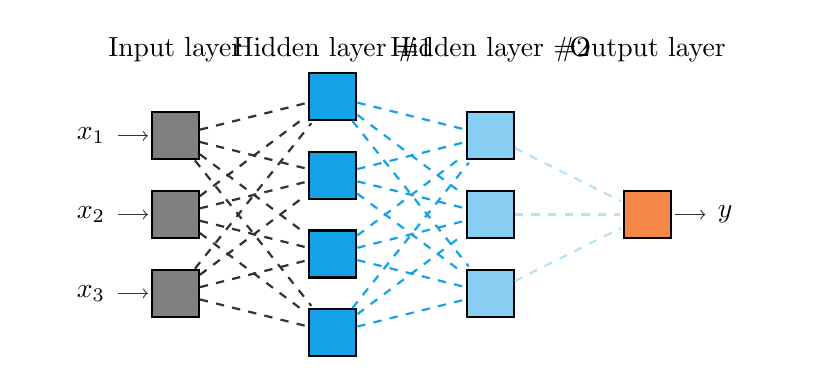
\begin{tikzpicture}[shorten >=1pt,-, draw=black!80, node distance=\layersep]
	\tikzstyle{every pin edge}=[<-,shorten <=1pt]
	\tikzstyle{neuron}=[draw=black, thick, rectangle, minimum size=17pt, inner sep=0pt, thick]
	% \tikzstyle{neuron}=[square, minimum size=17pt, inner sep=0pt, thick]
	\tikzstyle{input neuron}=[neuron, fill=Gray];
	\tikzstyle{output neuron}=[neuron, fill=Peach];
	\tikzstyle{hidden neuron}=[neuron, fill=Cerulean];
	\tikzstyle{hidden neuron2}=[neuron, fill=Cerulean!50];
	\tikzstyle{annot} = [text width=10em, text centered]


	% Draw the input layer nodes
	\foreach \name / \y in {1,...,3}
	% This is the same as writing \foreach \name / \y in {1/1,2/2,3/3,4/4}
	\node[input neuron, pin=left:$x_\y$] (I-\name) at (0,-\y) {};

	% Draw the hidden layer nodes
	\foreach \name / \y in {1,...,4}
	\path[yshift=0.5cm]
	node[hidden neuron] (H-\name) at (\layersep,-\y cm) {};

	% Draw the hidden layer nodes
	\foreach \name / \y in {1,...,3}
	\path[yshift=0.0cm]
	node[hidden neuron2] (H2-\name) at (\layersep+\layersep,-\y cm) {};

	% Draw the output layer node
	\node[output neuron,pin={[pin edge={->}]right:$y$}, right of=H2-2] (O) {};

	% Connect every node in the input layer with every node in the
	% hidden layer.
	\foreach \source in {1,...,3}
	\foreach \dest in {1,...,4}
	\path (I-\source) edge[thick,-,dashed] (H-\dest);
	% \path[path fading=fade IH1, thick, dashed, draw=Gray] (I-\source) -- (H-\dest);


	\foreach \source in {1,...,4}
	\foreach \dest in {1,...,3}
	\path (H-\source) edge[thick,-,dashed,draw=Cerulean] (H2-\dest);
	% \path[path fading=fade H1H2, thick, dashed, draw=Gray] (H-\source) -- (H2-\dest);

	% Connect every node in the hidden layer with the output layer
	\foreach \source in {1,...,3}
	\path (H2-\source) edge[thick,-,dashed,draw=Cerulean!30] (O);
	% \path[path fading=fade H2O, thick, dashed, draw=Gray] (H2-\source) -- (O);

	% Annotate the layers
	\node[annot,above of=H-1, node distance=0.6cm] (hl) {Hidden layer \#1};
	\node[annot,right of=hl] (hl2) {Hidden layer \#2};
	\node[annot,left of=hl] {Input layer};
	\node[annot,right of=hl2] {Output layer};
	\end{tikzpicture}
\end{figure}


    % \todo{output layers + regularization + works}
    Particular attention must be paid when fitting deep models as they can be prone to overfit the training set~\cite{angermueller2016deep}.
    The network topology itself defines the \textit{degrees of freedom} of the model: deeper and wider networks can approximate well very complicated input-output relationship, but also the noise affecting the data.
    Although, tuning the number of hidden layers and their size is not the recommended strategy to prevent from overfitting, as it may lead to suboptimal solutions.

    Regularization in MLPs can be controlled by penalizing the weights of the network (see Section~\ref{subsec:regularization_penalties}). The most common regularization strategy consists in adding an $\ell_2$-norm penalty in the objective function, as in Equation~\eqref{eq:losspen}. In the DL community this procedure is known as weight decay~\cite{krogh1992simple}.

    This strategy is adopted in \cite{Chen2015TransspeciesLO} to train a deep architecture on rat cell responses to given stimuli with the final aim to predict human cell responses in the same conditions.
    Moreover, weight decay is also adopted in \cite{Yuan2016DeepGeneAA} to train \textit{DeepGene}, \ie an MLP which is designed to classify the tumor type from a set of somatic point mutations.
    Furthermore, weight decay is used in~\cite{Fakhry2016DeepMF} to train a DL architecture for brain electron microscopy image segmentation.
    Although less common, the $\ell_1$-norm can also be adopted as regularization penalty, as in~\cite{leung2014deep}.

    Training MLPs, and deep networks in general, consists in solving a minimization problem via suitable optimization algorithms~\cite{ruder2016overview}. All these methods iteratively update the weights of the network in order to decrease the training error. A popular regularization strategy, known as  \textit{Early stopping}~\cite{prechelt1998early}, consists in interrupting the fitting process as soon as the error on an external validation set increases~\cite{angermueller2016deep}.

    Another common regularization strategy in DL is \textit{Dropout}~\cite{srivastava2014dropout}. This techniques consists in temporarily deactivating a defined number of randomly chosen units of the network at training phase. This reduces the degrees of freedom of the model and it implicitly allows to achieve an ensemble of several smaller networks whose predictions are combined.
    The use of dropout alone can improve the generalization properties, as in~\cite{Chen2016GeneEI}, where the authors propose a \textit{D-GEX}, DL regression architecture trained to predict the expression of a number of target genes. Dropout can also be used in combination with weight decay or other forms of regularization, as in~\cite{leung2014deep}, where the authors propose to use a deep network to achieve splicing pattern prediction.

	\begin{table}[htb]
		\centering
		\caption{Overview of the matrix norms used for multiple-output regression.}\label{tab:norms}
		\begin{tabular}{l|l|l}
			\toprule
			Matrix norm  & Notation         & Definition                      \\  \midrule
			Frobenius        & $\norm{A}_F$     & $\sqrt{\text{trace}(A^TA)}$     \\ [0.05cm]
			Nuclear          & $\norm{A}_*$     & $\text{trace}\sqrt{(A^TA)}$     \\ [0.05cm]
			Mixed $\text{L}_{2,1}$        & $\norm{A}_{2,1}$ & $\sum_{j}\norm{\bm{a}_j}_2$ \\ \bottomrule
		\end{tabular}
	\end{table}




  \section{Unsupervised learning} \label{subsec:unsupervised_learning}
    \subsection{Manifold learning}
    \subsection{Clustering}

  \section{Feature selection} \label{subsec:feature_selection}

  \section{Model selection and evaluation} \label{subsec:model_selection}
    \subsection{Model selection strategies}
    % cross validation flavours
    \subsection{Feature selection stability}
    % stability selection
    \subsection{Performance metrics}
    % sup and unsup
    % acc, f1, mcc, ...


\section{Computational requirements and implementations} \label{sec:implementation}
\begin{itemize}
  \item MPI
  \item GPU and accelerators
\end{itemize}
